\section{Projects guide} \label{s:platform-user-guide:projects}
	Projects can be created from the project tab available in left expander panel. Figure \ref{fig:project-list-view} shows the list of projects and button that creates new project.
	\begin{figure}[!htbp]
		\centering
		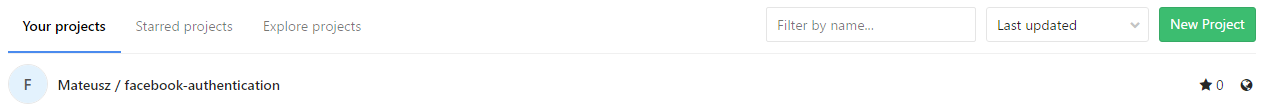
\includegraphics[width=1\textwidth]{img/ug-project/new-project2}
		\caption{Project list view.}
		\label{fig:project-list-view}
	\end{figure}
	After clicking on create project button user will be redirected to another view where all the necessary data will be displayed -- Figure \ref{fig:project-settings}. user can choose visibility of the project, description, name and additionally choose import settings for example from \emph{GitHub} or \emph{BitBucket} repositories. 
	\begin{figure}[!htbp]
		\centering
		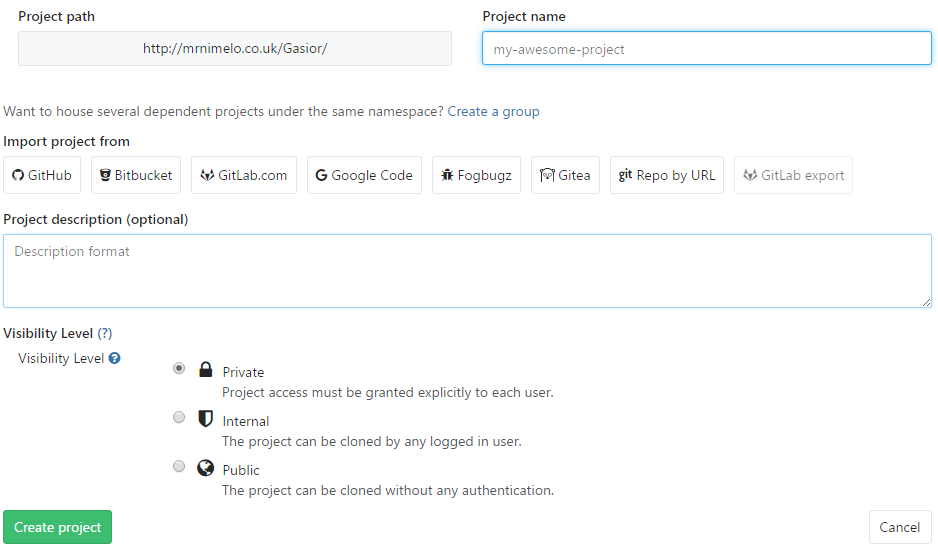
\includegraphics[width=1\textwidth]{img/ug-project/new-project-settings}
		\caption{New project settings panel.}
		\label{fig:project-settings}
	\end{figure}
	After creating the project there will be available new panel with permission as is shown in Figure \ref{fig:project-members-permissions}. Access to this panel is available from the gear situated in right top corner. User should be able to specify access to the users and groups with access level as well as the expiration date.
	\begin{figure}[!htbp]
		\centering
		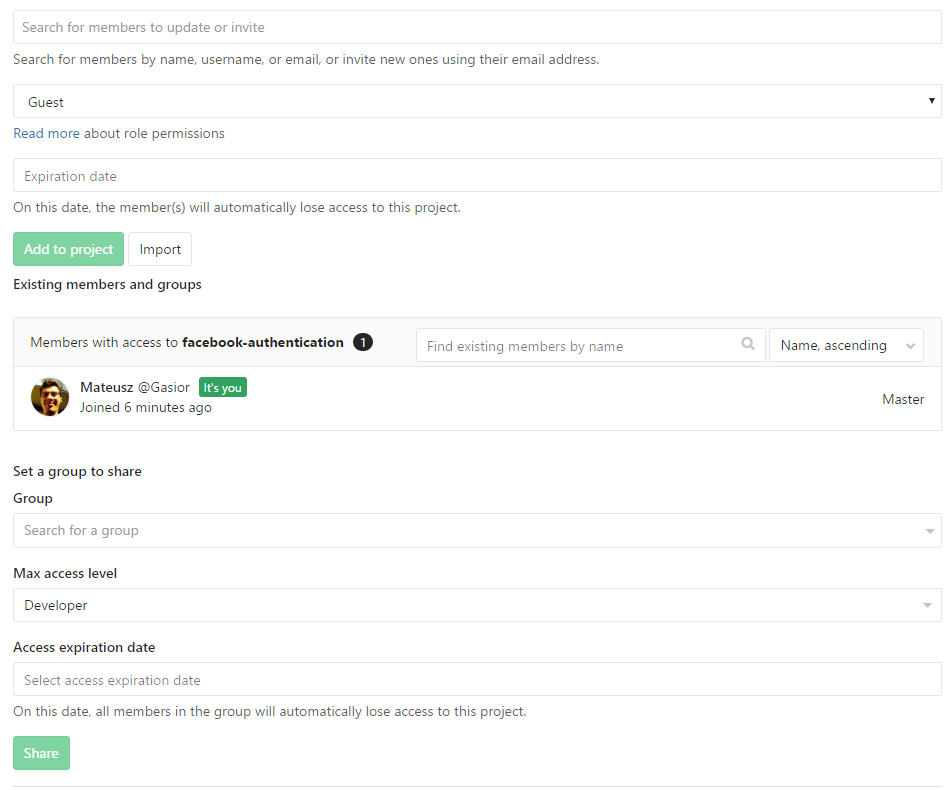
\includegraphics[width=1\textwidth]{img/ug-project/project-members-permissions}
		\caption{Project permissions panel.}
		\label{fig:project-members-permissions}
	\end{figure}
	User can see the details of the project by choosing project name from the projects available from the left expander panel -- Figure \ref{fig:project-view-panel}.
	\begin{figure}[!htbp]
		\centering
		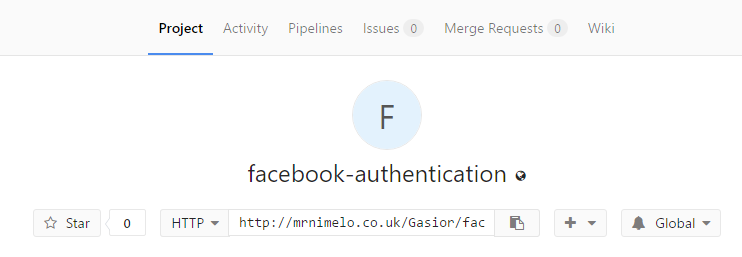
\includegraphics[width=1\textwidth]{img/ug-project/project-view}
		\caption{Project view panel.}
		\label{fig:project-view-panel}
	\end{figure}
	From the repository tab inside the project user can creates and upload file via web-browser as is shown in Figure \ref{fig:project-repository}.
	\begin{figure}[!htbp]
		\centering
		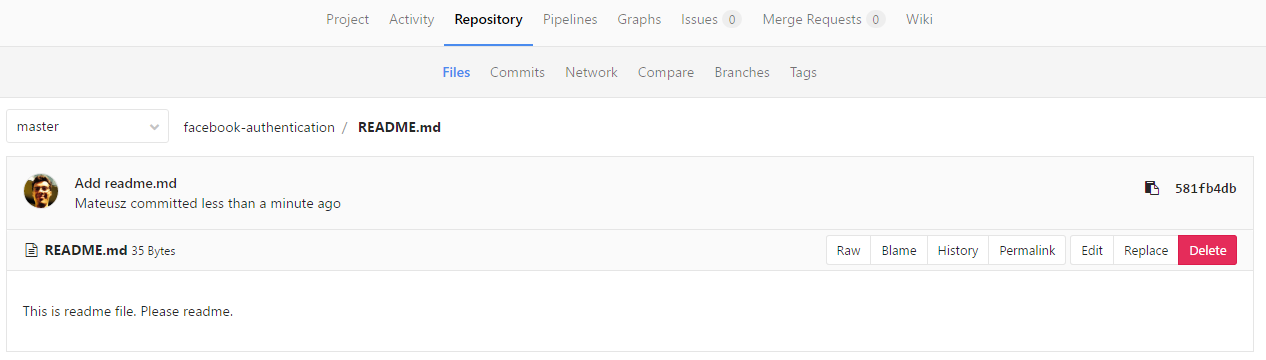
\includegraphics[width=1\textwidth]{img/ug-project/project-view2}
		\caption{Project repository view.}
		\label{fig:project-repository}
	\end{figure}
	From the member tab user can modify accesses and members/groups within the project -- Figure \ref{fig:project-members}.
	\begin{figure}[!htbp]
		\centering
		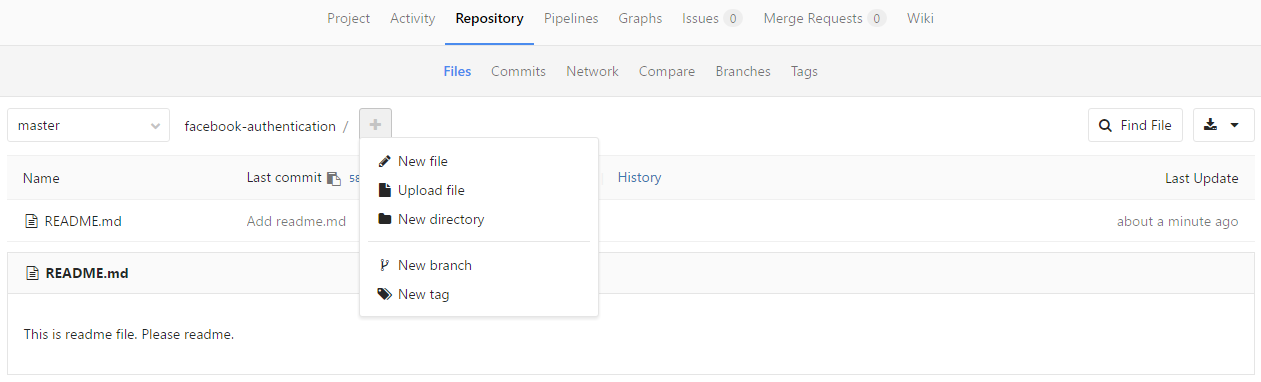
\includegraphics[width=1\textwidth]{img/ug-project/project-view-repository}
		\caption{Project members view panel.}
		\label{fig:project-members}
	\end{figure}